% ------------------------------------------------------------------------------------------
\begin{frame}
  \frametitle{Baumautomaten: Grundbegriffe}

  Betrachten \Bmph{unendlichen vollständigen Binärbaum}
  \begin{Itemize}
    \item
      Positionen: \emph{alle} Wörter aus $\{0,1\}^*$
    \item
      jeder Knoten $p$ hat linkes und rechtes Kind: $p0,p1$
    \item
      \Bmph{Tiefe} von Knoten $p$:\quad $|p|$
    \item
      \Bmph{Ebene} $k$: alle Knoten der Tiefe $k$
    \item
      $p_2$ ist \Bmph{Nachfolger} von $p_1$, geschrieben $p_1 \sqsubseteq p_2$,\\
      wenn $p_2=p_1p$ für ein $p \in \{0,1\}^*$
      \Tafel
  \end{Itemize}

  \par\medskip
  \uncover<2->{%
    \Bmph{Pfad}: Teilmenge $\pi \subseteq \{0,1\}^*$ mit $\varepsilon \in \pi$ und:
    \begin{Itemize}
%           \item
%             Wurzel $\varepsilon \in \pi$
      \item
        wenn $p \in \pi$, dann genau eins der Kinder $p0,p1$ in $\pi$
      \item
        $\forall k$: von allen Knoten der Ebene $k$ ist genau einer in $\pi$ \\
        \TafelForts
    \end{Itemize}
  }

  \par%\medskip
  \uncover<3->{%
    \Bmph{$\Sigma$-Baum $t$} (Alphabet $\Sigma$ ohne Stelligkeit): \\
    \begin{Itemize}
      \item[]
        Funktion $t : \{0,1\}^* \to \Sigma$
        \TafelForts
    \end{Itemize}
  }

  \note{%
    \textbf{16:00}
    
    \par
  }
\end{frame}

%% ------------------------------------------------------------------------------------------
%\begin{frame}
%  \frametitle{Skizzen zu den Grundbegriffen}
%
%  Positionen und Pfade im Binärbaum
%  \begin{center}
%    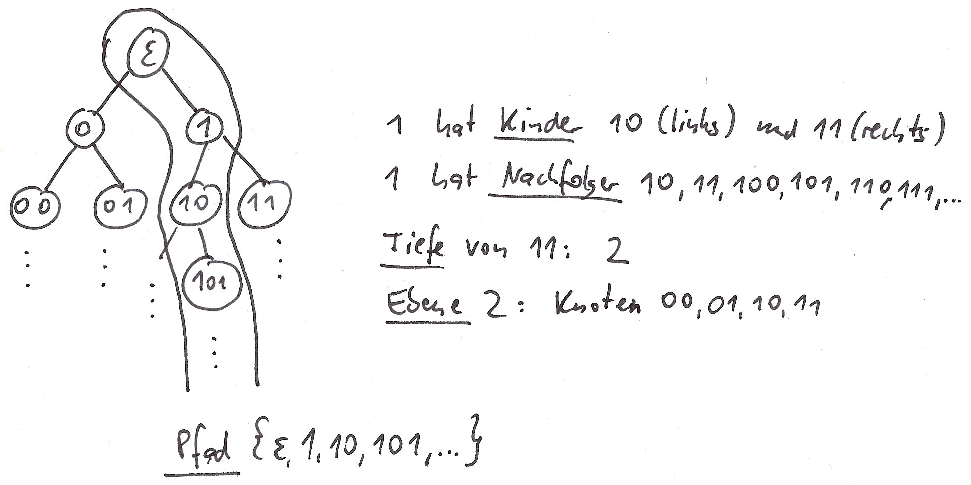
\includegraphics[scale=.5]{img/skizzen_baeume_1.pdf}
%  \end{center}
%
%  \par\bigskip
%%       Beispiel für einen $\Sigma$-Baum, $\Sigma=\{a,b\}$
%  Beispiel-$\Sigma$-Baum,\\
%  $\Sigma=\{a,b\}$
%  \par\vspace*{-2.1\baselineskip}
%  \hspace*{.3\textwidth}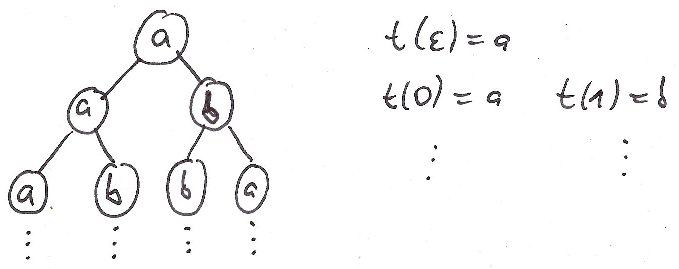
\includegraphics[scale=.5]{img/skizzen_baeume_2.pdf}
%
%  \note{~}
%\end{frame}

% ------------------------------------------------------------------------------------------
\begin{frame}
  \frametitle{Baumautomaten: etwas mehr Notation (1)}
  
  $\hat t = \Bmph{$t[p \to t_1]$}$:
  \par\smallskip
  der Baum, den man aus $t$ erhält, wenn man den Teilbaum,\\
  der in $p$ wurzelt, durch $t_1$ ersetzt

  \par\bigskip
  Skizze:
  \begin{center}
    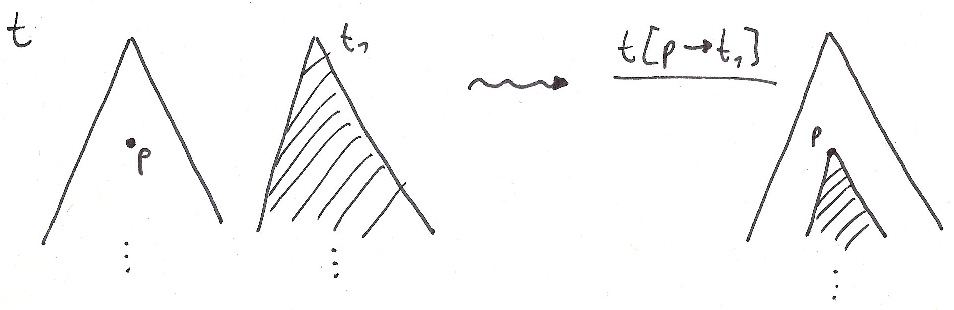
\includegraphics[scale=.5]{img/skizzen_baeume_3.pdf}
  \end{center}

  \par\bigskip
  exakte Beschreibung:
  \[
    \hat t(p') =
    \begin{cases}
      t_1(p'') & \text{wenn } p'=pp'' \\
      t(p')    & \text{wenn } p \not\sqsubseteq p'
    \end{cases}
  \]

  \note{%
    \textbf{16:08}
    
    \par
  }
\end{frame}

% ------------------------------------------------------------------------------------------
\begin{frame}
  \frametitle{Baumautomaten: etwas mehr Notation (2)}

  $\hat t = \Bmph{$a(t_0,t_1)$}$:
  \par\smallskip
  der Baum mit Wurzel $a$ und Teilbäumen $t_0,t_1$ in den Wurzelkindern $0,1$:

  \par\bigskip
  Skizze:
  \begin{center}
    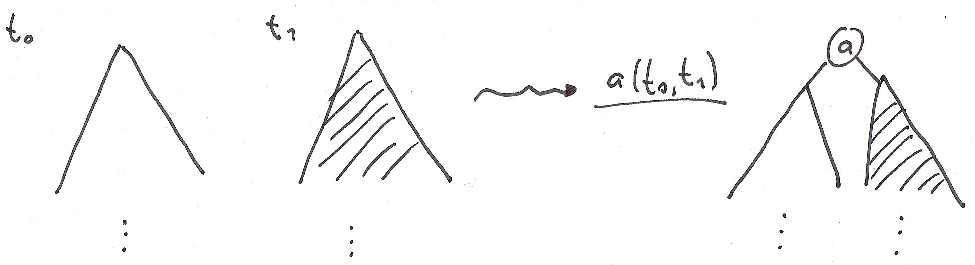
\includegraphics[scale=.5]{img/skizzen_baeume_4.pdf}
  \end{center}

  \par\bigskip
  exakte Beschreibung:
  \[
    \hat t(p) =
    \begin{cases}
      a        & \text{wenn } p=\varepsilon \\
      t_0(p')  & \text{wenn } p=0p'         \\
      t_1(p')  & \text{wenn } p=1p'
    \end{cases}
  \]

  \note{%
    \textbf{16:11}
    
    \par
  }
\end{frame}

% ------------------------------------------------------------------------------------------
\begin{frame}
  \frametitle{Baumautomaten: Definition}

  \begin{Definition}
    Ein \Bmph{nichtdeterministischer Büchi-Baumautomat (NBBA)} über $\Sigma$\\
    ist ein 5-$\!$Tupel
    $\Aut{A} = (Q, \Sigma, \Delta, I, F)$, wobei
    \begin{Itemize}
      \item
        $Q$ eine endliche nichtleere \Bmph{Zustandsmenge} ist,
      \item
        $\Sigma$ ein Alphabet ist
      \item
        $\Delta \subseteq Q \times \Sigma \times \uwave{Q \times Q}$ die \Bmph{Überführungsrelation} ist,
      \item
        $I \subseteq Q$ die Menge der \Bmph{Anfangszustände} ist,
      \item
        $F \subseteq Q$ die Menge der \Bmph{akzeptierenden Zustände} ist.
    \end{Itemize}
  \end{Definition}

  \par\bigskip
  \uncover<2->{%
    (entsprechen offenbar Top-down-Automaten)
  }

  \note{%
    \textbf{16:14}
    
    \par
  }
\end{frame}

% ------------------------------------------------------------------------------------------
\begin{frame}
  \frametitle{Muller- und Paritäts-Baumautomaten}

  \begin{Definition}
    Ein \Bmph{nichtdeterministischer Muller-Baumautomat (NMBA)} über $\Sigma$\\
    ist ein 5-$\!$Tupel
    $\Aut{A} = (Q, \Sigma, \Delta, I, \calF)$, wobei
    \begin{Itemize}
      \item
        $Q,\Sigma,\Delta,I$ wie für NBBAs sind
      \item
        $\calF \subseteq 2^Q$ die \Bmph{Akzeptanzkomponente} ist
    \end{Itemize}

    \par\bigskip
    \uncover<2->{%
      Ein \Bmph{nichtdeterministischer Paritäts-Baumautomat (NPBA)} über $\Sigma$\\
      ist ein 5-$\!$Tupel
      $\Aut{A} = (Q, \Sigma, \Delta, I, c)$, wobei
      \begin{Itemize}
        \item
          $Q,\Sigma,\Delta,I$ wie für NBBAs sind
        \item
          $c : Q \to \mathbb{N}$ die \Bmph{Akzeptanzkomponente} ist
      \end{Itemize}
    }
  \end{Definition}

  \par\bigskip
  \uncover<3->{%
    (Rabin- und Streett-Baumautomaten wie üblich definiert)
  }

  \note{%
    \textbf{16:15}
    
    \par
  }
\end{frame}

% ------------------------------------------------------------------------------------------
\begin{frame}
  \frametitle{Runs auf Baumautomaten}

  Run $=$ Markierung der Positionen in $\{0,1\}^*$ mit Zuständen,\\
  verträglich mit Anfangszuständen und Überführungsrelation

  \par\bigskip
  \uncover<2->{%
    \begin{Definition}
      Ein \Bmph{Run} eines NBBA (NMBA, NPBA) \Aut{A} auf einem $\Sigma$-Baum $t$\\
      ist eine Funktion $r : \{0,1\}^* \to Q$, so dass
      \begin{Itemize}
        \item
          $r(\varepsilon) \in I$;
        \item
          für alle $p \in \{0,1\}^*$ gilt: $\big(r(p), t(p), r(p0), r(p1)\big) \in \Delta$
      \end{Itemize}
    \end{Definition}
  }

  \par\bigskip
  \uncover<3->{%
    Erfolgreicher Run: verträglich mit Akzeptanzkomponente
  }

  \note{%
    \textbf{16:16}
    
    \par
  }
\end{frame}

%   \newlength{\leftbox}
%   \settowidth{\leftbox}{$x=\text{Parität}$;}
%   \newlength{\midbox}
%   \settowidth{\midbox}{$\textsl{Acc}=\calF$;}
%   % ------------------------------------------------------------------------------------------
%     \begin{frame}
%       \frametitle{Erfolgreiche Runs}
% 
%       Sei $r$ Run eines N$x$BAs \Aut{A} % auf einem $\Sigma$-Baum $t$
%       und $\pi$ ein Pfad
% 
%       \par\medskip
%       Betrachten wieder \Bmph{Unendlichkeitsmenge}
%       \[
%         \Inf(r,\pi) = \{q \in Q \mid r(p) = q \text{~für unendlich viele~} p \in \pi\}
%       \]
% 
%       \par%\bigskip
%       \begin{Definition}<2->      
%         Run $r$ des N$x$BA $\Aut{A}=(Q,\Sigma,\Delta,I,\textsl{Acc})$ ist \Bmph{erfolgreich}, falls
%         \begin{Itemize}
%           \item
%             \parbox{\leftbox}{$x=\text{Büchi}$;} \parbox{\midbox}{$\textsl{Acc}=F$;} für alle Pfade $\pi$:~
%             $
%               \Inf(r,\pi) \cap F \neq \emptyset
%             $
%           \item<3->
%             \parbox{\leftbox}{$x=\text{Muller}$;} \parbox{\midbox}{$\textsl{Acc}=\calF$;} für alle Pfade $\pi$:~
%             $
%               \Inf(r,\pi) \in \calF
%             $
%           \item<4->
%             \parbox{\leftbox}{$x=\text{Parität}$;} \parbox{\midbox}{$\textsl{Acc}=c$;} für alle Pfade $\pi$:
%             \[
%               \min\{c(q) \mid q \in \Inf(r,\pi)\} \text{~ist gerade}
%             \]%
%         \end{Itemize}
% 
%         \par\vspace*{-1.2\baselineskip}
%         \uncover<5->{%
%           $\Aut{A}$ \Bmph{akzeptiert} $t$, wenn es einen erfolgreichen Run von \Aut{A} auf $t$ gibt.
%         }
% 
%         \par\smallskip
%         \uncover<6->{%
%           \Bmph{$L_\omega(\Aut{A})$} $=$ $\{t \mid \Aut{A} \text{~akzeptiert~} t\}$
%         }
%       \end{Definition}
% 
%       \note{~}
%     \end{frame}

% ------------------------------------------------------------------------------------------
\begin{frame}
  \frametitle{Erfolgreiche Runs}

  Sei $r$ Run eines N$x$BAs \Aut{A} % auf einem $\Sigma$-Baum $t$
  und $\pi$ ein Pfad

  \par\smallskip
  Betrachten wieder \Bmph{Unendlichkeitsmenge}
  \[
    \Inf(r,\pi) = \{q \in Q \mid r(p) = q \text{~für unendlich viele~} p \in \pi\}
  \]

  \par
  \begin{Definition}<2->      
    \begin{Itemize}
      \item
        Run $r$ des NBBA $\Aut{A}=(Q,\Sigma,\Delta,I,F)$ ist \Bmph{erfolgreich}, falls
        \par\smallskip
        \Emph{für alle Pfade} $\pi$ gilt:~ $\Inf(r,\pi) \cap F \neq \emptyset$
        \par\smallskip
      \item<3->
        Run $r$ des NMBA $\Aut{A}=(Q,\Sigma,\Delta,I,\calF)$ ist \Bmph{erfolgreich}, falls
        \par\smallskip
        \Emph{für alle Pfade} $\pi$ gilt:~ $\Inf(r,\pi) \in \calF$
        \par\smallskip
      \item<4->
        Run $r$ des NPBA $\Aut{A}=(Q,\Sigma,\Delta,I,c)$ ist \Bmph{erfolgreich}, falls
        \par\smallskip
        \Emph{für alle Pfade} $\pi$ gilt:~ 
        $
          \min\{c(q) \mid q \in \Inf(r,\pi)\} \text{~ist gerade}
        $
    \end{Itemize}

%         \par\vspace*{-1.2\baselineskip}
  \end{Definition}

  \note{%
    \textbf{16:18}
    
    \parI
    Parity-Bedingung: in Aufgabe 4 auf Übungsblatt 4 war es max statt min \\
    -- macht aber keinen Unterschied; ggf.\ Nummerierung der Zustände "`umdrehen"'.
    
    \par
  }
\end{frame}

% ------------------------------------------------------------------------------------------
\begin{frame}
  \frametitle{Akzeptanz und erkannte Sprache}

  \dots\ sind wie üblich definiert:

  \par\bigskip
  \begin{Definition}
    Sei $\Aut{A}$ ein NBBA, NMBA oder NPBA,\\
    sei $t$ ein $\Sigma$-Baum und $L$ eine Menge von $\Sigma$-Bäumen.
    \begin{Itemize}
      \item
        $\Aut{A}$ \Bmph{akzeptiert} $t$,\\
        wenn es einen erfolgreichen Run von \Aut{A} auf $t$ gibt.
        \par\smallskip
      \item
        \Bmph{$L_\omega(\Aut{A})$} $=$ $\{t \mid \Aut{A} \text{~akzeptiert~} t\}$
        \par\bigskip
      \item
        $L$ heißt \Bmph{Büchi-erkennbar},\\
        wenn es einen NBBA $\Aut{A}$ gibt mit $L_\omega(\Aut{A})=L$.
        \par\smallskip
      \item
        Analog: \Bmph{Muller-erkennbar} und \Bmph{paritäts-erkennbar}
    \end{Itemize}
  \end{Definition}

  \note{%
    \textbf{16:20}
    
    \par
  }
\end{frame}

% ------------------------------------------------------------------------------------------
\begin{frame}
  \frametitle{Beispiele (Büchi)}

  \begin{Itemize}
    \item<+->
      NBBA $\Aut{A}=(\{A,B\},~\{a,b\},~\Delta,~\{A\},~\{A\})$ mit %\Tafel
      \[
        \Delta = \{~(A,a,A,A),~(B,a,A,A),~(A,b,B,B),~(B,b,B,B)~\}
      \]
      Skizze:
      \par\vspace*{-\baselineskip}
      \begin{center}
        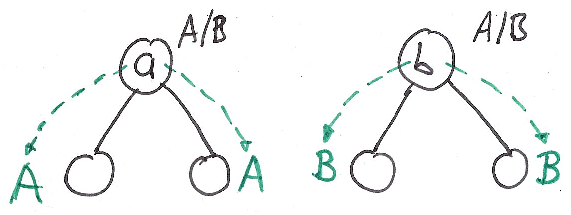
\includegraphics[scale=.5]{img/beispielautomaten_1.pdf}
      \end{center}

      \par\bigskip
      $L_\omega(\Aut{A})$ $=$
      \only<.|handout:0>{?}%
      \uncover<+->{$\{t \mid \text{jeder Pfad hat $\infty$ viele $a$'s}\}$}
      \par\bigskip
    \item<+->
      derselbe NBBA, aber mit $F=\{B\}$
      \par\smallskip
      $L_\omega(\Aut{A})$ $=$
      \only<.|handout:0>{?}%
      \uncover<+->{$\{t \mid \text{jeder Pfad hat $\infty$ viele $b$'s}\}$}
      \par\bigskip
    \item<+->
      derselbe NBBA, aber mit $F=\{A,B\}$
      \par\smallskip
      $L_\omega(\Aut{A})$ $=$
      \only<.|handout:0>{?}%
      \uncover<+->{$\{t \mid t \text{~ist ein $\Sigma$-Baum}\}$}
  \end{Itemize}

  \note{%
    \textbf{16:21}
    
    \par
  }
\end{frame}

% ------------------------------------------------------------------------------------------
\begin{frame}
  \frametitle{Beispiele (Büchi)}

  \begin{Itemize}
    \item<+->
      NBBA $\Aut{A}=(\{A,B,X\},~\{a,b\},~\Delta,~\{A\},~\{A,X\})$ mit $\Delta = $%\Tafel
%           \[
%             \begin{array}{rlll}
%               \text{mit~} \Delta = \{~ & (A,a,A,X),~ & (A,a,X,A), & \\
%                                        & (B,a,A,X),~ & (B,a,X,A), & \\[5pt]
%                                        & (A,b,B,X),~ & (A,b,X,B), & \\
%                                        & (B,b,B,X),~ & (B,b,X,B), & \\[5pt]
%                                        & (X,a,X,X),~ & (X,b,X,X)~ & \}
%             \end{array}
%           \]
      \par\medskip
      \begin{small}
        \mbox{$
          \begin{array}{@{}r@{~}l@{~~}l@{~~}l@{~~}l@{~~}l@{~}l@{}}
            \{ & (A,a,A,X),~ & (B,a,A,X),~ & (A,b,B,X),~ & (B,b,B,X),~ & (X,a,X,X), &    \\
               & (A,a,X,A),~ & (B,a,X,A),~ & (A,b,X,B),~ & (B,b,X,B),~ & (X,b,X,X)  & \}
          \end{array}
        $\hspace*{-10mm}}

        \par\smallskip
        Skizze:
        \par\vspace*{-\baselineskip}
        \begin{center}
          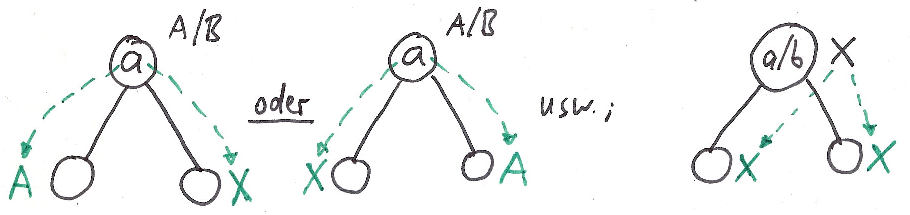
\includegraphics[scale=.5]{img/beispielautomaten_2.pdf}
        \end{center}
      \end{small}

      \par\smallskip
      $L_\omega(\Aut{A})$ $=$
      \only<.|handout:0>{?}%
      \uncover<+->{$\{t \mid \text{$t$ hat mind.\ einen Pfad mit $\infty$ vielen $a$'s}\}$}
      \par\bigskip
    \item<+->
      derselbe NBBA, aber mit $F=\{B,X\}$
      \par\smallskip
      $L_\omega(\Aut{A})$ $=$
      \only<.|handout:0>{?}%
      \uncover<+->{$\{t \mid \text{$t$ hat mind.\ einen Pfad mit $\infty$ vielen $b$'s}\}$}
      \par\bigskip
    \item<+->
      derselbe NBBA, aber mit $F=\{X\}$%
      \uncover<7->{:\qquad $L_\omega(\Aut{A}) = \emptyset$}
      \par\smallskip
      \only<5-6|handout:0>{$L_\omega(\Aut{A})$ $=$ }%
      \only<5|handout:0>{?}%
      \only<6|handout:0>{$\emptyset$}%
%           \par\medskip
    \item<7->
      derselbe NBBA, aber mit $F=\{A,B\}$%
%           \uncover<0|handout:1>{:\hfill $L_\omega(\Aut{A}) = \emptyset$}
%           \par\smallskip
      \only<7-8|handout:0>{:\quad $L_\omega(\Aut{A})$ $=$ }%
      \only<7|handout:0>{?}%
      \only<8|handout:0>{$\emptyset$}%
      \uncover<0|handout:1>{\phantom{$()$}}%
  \end{Itemize}%
  \alt<1-4,7-8|handout:1>{\vspace*{-3.2pt}}{\vspace*{-16.8pt}}%

  \note{%
    \textbf{16:24}
    
    \parII
    1.\ Bsp.:~ lies \textbf{spaltenweise!}
    
    \par
  }
\end{frame}

% ------------------------------------------------------------------------------------------
\begin{frame}
  \frametitle{Beispiele (Muller)}
  \label{fra:beispiele_muller}

  \begin{Itemize}
    \item<+->
      NMBA $\Aut{A}=(\{A,B\},~\{a,b\},~\Delta,~\{A\},~\{\{A\}\})$ mit %\Tafel
      \[
        \Delta = \{~(A,a,A,A),~(B,a,A,A),~(A,b,B,B),~(B,b,B,B)~\}
      \]
      Skizze:
      \par\vspace*{-1.4\baselineskip}
      \begin{center}
        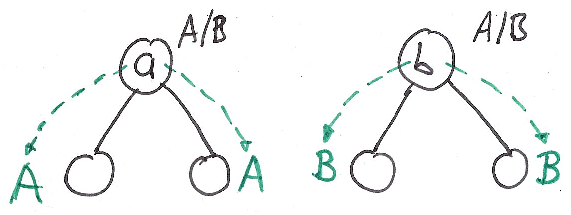
\includegraphics[scale=.45]{img/beispielautomaten_1.pdf}
      \end{center}

      \par\vspace*{-.4\baselineskip}
      $L_\omega(\Aut{A})$ $=$
      \only<.|handout:0>{?}%
      \uncover<+->{$\{t \mid \text{jeder Pfad hat endlich viele $b$'s}\}$ (!)}
      \par\medskip
    \item<+->
      derselbe NMBA, aber mit $F=\{\{B\}\}$
      \par\smallskip
      $L_\omega(\Aut{A})$ $=$
      \only<.|handout:0>{?}%
      \uncover<+->{$\{t \mid \text{jeder Pfad hat endlich viele $a$'s}\}$}
      \par\medskip
    \item<+->
      derselbe NMBA, aber mit $F=\{\{A,B\}\}$
      \par\smallskip
      $L_\omega(\Aut{A})$ $=$
      \only<.|handout:0>{?}%
      \uncover<+->{$\{t \mid \text{jeder Pfad hat $\infty$ viele $a$'s und $\infty$ viele $b$'s}\}$}
      \par\medskip
    \item<+->
      derselbe NMBA, aber mit $F=\{\{A\},\{B\}\}$
      \par\smallskip
      $L_\omega(\Aut{A})$ $=$
      \mbox{%
        \only<.|handout:0>{?}%
        \uncover<+->{$\{t \mid \text{jeder Pfad hat endl.\ viele $b$'s \emph{oder} endl.\ viele $a$'s}\}$}%
        \hspace*{-5mm}%
      }
  \end{Itemize}

  \note{%
    \textbf{16:28}
    
    \par
  }
\end{frame}
  
% ------------------------------------------------------------------------------------------
\begin{frame}
  \frametitle{Beispiel (Parität)}

    \Bmph{Zur Erinnerung:}
    \par\smallskip
    \begin{block}{}
      Run $r$ ist erfolgreich, wenn für alle Pfade $\pi \subseteq T$ gilt:
      \[
        \min\{c(q) \mid q \in \Inf(r,\pi)\} \text{~ist gerade}
      \]      
    \end{block}

    \par\bigskip
    \uncover<2->{%
      NPBA $\Aut{A}=(\{A,B\},~\{a,b\},~\Delta,~\{A\},~c)$ mit %\Tafel
      %
      \begin{align*}
        \Delta & = \{~(A,a,A,A),~(B,a,A,A),~(A,b,B,B),~(B,b,B,B)~\} \\[4pt]
        c(A)   & = 1                                                \\
        c(B)   & = 2
      \end{align*}
      %
      \vspace*{-4.4\baselineskip}
      \begin{center}
        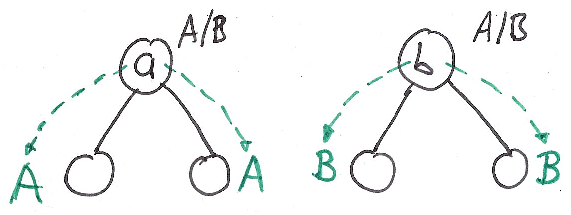
\includegraphics[scale=.45]{img/beispielautomaten_1.pdf}
      \end{center}
      %
      $L_\omega(\Aut{A})$ $=$
      \only<2|handout:0>{?}%
      \uncover<3>{$\{t \mid \text{jeder Pfad hat endlich viele $a$'s}\}$}
    }

  \note{%
    \textbf{16:32}
        
    \par
  }
\end{frame}

%% ------------------------------------------------------------------------------------------
%\begin{frame}
%  \frametitle{Büchi- versus Muller-Erkennbarkeit}
%  
%  \begin{Satz}
%    \begin{Enumerate}
%      \item
%        Jede Büchi-erkennbare Sprache ist Muller-erkennbar.
%      \item
%        \Emph{Nicht jede} Muller-erkennbare Sprache ist Büchi-erkennbar.
%    \end{Enumerate}
%    \label{thm:buchi_vs_muller}
%    \par\vspace*{-.4\baselineskip}
%  \end{Satz}
%
%  \par\medskip
%  \uncover<2->{%
%    \Bmph{Beweis.}
%    \begin{Enumerate}
%      \item
%        Wie im letzten Kapitel.
%      \item<3->
%        Idee:
%        \begin{Itemize}
%          \item
%            Betrachten $L = \{t \mid \text{jeder Pfad in $t$ hat endlich viele $a$'s}\}$;\\
%            nehmen an, $L$ werde von NBBA $\Aut{A}$ mittels Run $r$ erkannt
%          \item
%            Bestimme Baum $t \in L$ und Pfad, auf dem zwischen zwei Besuchen
%            \emph{desselben} akzeptierenden Zustandes ein $a$ auftritt
%          \item
%            "`Pumpe"' $t,r$ so auf, dass dieser Teilpfad sich $\infty$ oft wiederholt
%          \item[\dred{\lightning}]
%            Neuer Baum wird akzeptiert, aber neuer Pfad hat $\infty$ viele $a$'s
%        \end{Itemize}
%        \par\smallskip
%        Details: s.\ Tafel \Tafel~~~~
%    \end{Enumerate}
%  }
%  \uncover<3->{%
%    \par\vspace*{-1.3\baselineskip} \qed%
%  }
%
%  \note{%
%    \textbf{16:35 bis 16:55, 5\,min Pause}
%    
%    \parI
%    TODO:~ mehr vom Beweishergang auf Folie tun, weniger Tafelanschrieb!
%    
%    \par
%  }
%\end{frame}
%
% ------------------------------------------------------------------------------------------
\begin{frame}
  \frametitle{Büchi- versus Muller-Erkennbarkeit}
  
  \begin{Satz}
    \begin{Enumerate}
      \item
        Jede Büchi-erkennbare Sprache ist Muller-erkennbar.
      \item
        \Emph{Nicht jede} Muller-erkennbare Sprache ist Büchi-erkennbar.
    \end{Enumerate}
    \label{thm:buchi_vs_muller}
    \par\vspace*{-.4\baselineskip}
  \end{Satz}

  \par\medskip
  \uncover<2->{%
    \Bmph{Beweis.}
    \begin{Enumerate}
      \item
        Wie im letzten Kapitel.
        \par\medskip
      \item<3->
        Betrachten $L = \{t \mid \text{jeder Pfad in $t$ hat endlich viele $a$'s}\}$
        \par\medskip
        $L$ ist Muller-erkennbar (siehe Bsp.\ auf Folie~\ref{fra:beispiele_muller})
        \par\medskip
        Müssen zeigen: $L$ nicht Büchi-erkennbar
    \end{Enumerate}
  }

  \note{%
    \textbf{16:35}
    
    \par
  }
\end{frame}

% ------------------------------------------------------------------------------------------
\begin{frame}
  \frametitle{Büchi- versus Muller-Erkennbarkeit}
  
  \Bmph{Zu zeigen:}~~
  $L = \{t \mid \text{jeder Pfad in $t$ hat endlich viele $a$'s}\}$ \\
  nicht Büchi-erkennbar.
  
  \par\bigskip
  \uncover<2->{%
    Nehmen an, es gebe NBBA $\Aut{A} = (Q,\Sigma,\Delta,I,F)$ mit $L_\omega(\Amc) = L$.
  }
  
  \par\medskip
  \uncover<3->{%
    O.\,B.\,d.\,A.\ sei $I = \{q_0\}$.\qquad Sei $n := |F|$.
  }
  
  \par\bigskip
  \uncover<4->{%
    \Bmph{Idee:}~
    %
    \begin{Itemize}
      \item
        Bestimme Baum $t \in L$ mit Run $r$ und Pfad, auf dem zwischen 2~Besuchen
        \emph{desselben} akzeptierenden Zustandes ein $a$ auftritt
      \item
        "`Pumpe"' $t,r$ so auf, dass dieser Teilpfad sich $\infty$ oft wiederholt
      \item[\dred{\lightning}]
        Neuer Baum wird akzeptiert, aber neuer Pfad hat $\infty$ viele $a$'s
    \end{Itemize}
  }

  \note{%
    \textbf{16:36}
    
    \par
  }
\end{frame}

% ------------------------------------------------------------------------------------------
\begin{frame}
  \frametitle{Büchi- versus Muller-Erkennbarkeit}

  Betrachte Baum $t \in L$ mit
  \hfill
  $
    t(p) = a \quad\text{gdw.}\quad p \in \displaystyle\bigcup_{i=1,\dots,n} (1^+0)^i,
  $
  
  \par\medskip
  \uncover<2->{%
    d.\,h.\ $t$ enthält ein $a$ an allen Positionen, die man erreicht, \\
    wenn man bei der Wurzel startet und bis zu $n$-mal wie folgt läuft:
    %
    \begin{itemize}
      \item
        einmal oder mehrmals zum rechten Kind (beliebig oft)
      \item
        einmal zum linken Kind\quad ("`Linksschritt"')
    \end{itemize}
  }
  %
  \uncover<3->{%
    An den übrigen Positionen enthält $t$ ein $b$.
  }
  
  \par\medskip
  \uncover<4->{%
    \Bmph{Skizze:}
    \qquad
    \begin{tikzpicture}[%
      node distance=12mm,>=Latex,baseline=-4pt,
      every node/.style={circle,draw=none,fill=none,inner sep=.4mm,minimum size=4mm},
      every edge/.style={draw=black,thick}
    ]
      \node (00)                                {\footnotesize $b$};
      \node[below right=0mm and 3mm of 00] (01) {\footnotesize $b$};
      \node[below right=0mm and 3mm of 01] (02) {\footnotesize $b$};
      \node[below left =0mm and 3mm of 02] (10) {\small \Emph{$a$}};
      \node[below right=0mm and 3mm of 10] (11) {\footnotesize $b$};
      \node[below right=0mm and 3mm of 11] (12) {\footnotesize $b$};
      \node[below left =0mm and 3mm of 12] (20) {\small \Emph{$a$}};
      \node[below right=0mm and 3mm of 20] (21) {};
      
      \path[-]
        (00) edge (01)
        (01) edge[draw=none] node [sloped,pos=.6] {\scalebox{.8}[1]{{\footnotesize $\cdots$}}} (02)
        (02) edge (10)
        (10) edge (11)
        (11) edge[draw=none] node [sloped,pos=.6] {\scalebox{.8}[1]{{\footnotesize $\cdots$}}} (12)
        (12) edge (20)
        (20) edge[draw=none] node [sloped,pos=.6] {\scalebox{.8}[1]{{\footnotesize $\cdots$}}} (21)
        ;
    \end{tikzpicture}
    %
%    \raisebox{-2.5\baselineskip}{%
    \raisebox{-.7\baselineskip}{%
      $\left.\rule{0pt}{1.4\baselineskip}\right\}$
      \begin{tabular}{@{}l@{}}
        bis zu \\
        $n$-mal
      \end{tabular}
    }%
  }
  
  \par\medskip
  \uncover<5->{%
    Klar:~ $t \in L$.\qquad Sei $r$ ein erfolgreicher Run.
  }

  \par\medskip
  \uncover<6->{%
    Details des Pumpens: s.\ Tafel \Tafel~~~~
    \par\vspace*{-\baselineskip} \qed%
  }

  \note{%
    \textbf{16:38 bis 16:50, 5\,min Pause}
    
    \parI
    Man beachte:~ $a$'s tauchen in \emph{beliebiger Tiefe} auf, \\
    aber auf jedem Pfad nur auf den ersten $n$ Linksschritten.
    
    \parI
    Dadurch hat jeder Pfad nur max.\ $n$ $a$'s, also endlich viele.
    
    \par
  }
\end{frame}

% ------------------------------------------------------------------------------------------
\begin{frame}
  \frametitle{Folgerung aus dem Beweis von Satz \ref{thm:buchi_vs_muller}}

  \begin{Folgerung}
    Die Klasse der Büchi-erkennbaren Baumsprachen ist\\
    \Emph{nicht} abgeschlossen unter
    \only<1|handout:0>{?}%
    \uncover<2->{Komplement.}
    \label{cor:Buchi_erkennbar_nicht_unter_Komplement_abgeschlossen}
  \end{Folgerung}

  \par\bigskip
  \uncover<3->{%
    Man kann Satz \ref{thm:buchi_vs_muller} stärker formulieren (ohne Beweis):

    \par\medskip
    \begin{Satz}
      Die Menge der Baumsprachen, die Muller-, aber nicht Büchi-erkennbar sind, ist
      \[
        \{L_\triangle \mid L \text{ ist NBA-erkennbar, aber nicht DBA-erkennbar}\}.
      \]
    \end{Satz}
  }

  \par\medskip
  \uncover<3->{%

    \begin{small}
      ($L \subseteq \Sigma^\omega$ ist eine $\omega$-Sprache;
      \par\smallskip
      $L_\triangle$ $=$ Menge aller $\Sigma$-Bäume,
      deren Beschriftung entlang \emph{jedes} Pfades in $L$ \\
      \hspace*{\fill} liegt)
      \par
    \end{small}
  }

  \note{%
    \textbf{16:55}
    
    \parI
    \textbf{Vor Satz 4.14 sagen:}~ Anfang des letzten Beweises erinnert nicht ohne Grund
    an Beweis der Ungleichmächtigkeit von DBAs und NBAs
    
    \par
  }
\end{frame}

% ------------------------------------------------------------------------------------------
\begin{frame}
  \frametitle{Paritäts- versus Muller-Erkennbarkeit}

  \begin{Satz}
    \begin{Enumerate}
      \item
        Jede paritäts-erkennbare Sprache ist Muller-erkennbar.
      \item
        Jede Muller-erkennbare Sprache ist paritäts-erkennbar.
    \end{Enumerate}
    \label{thm:muller_vs_paritaet}
    \par\vspace*{-.2\baselineskip}
  \end{Satz}

  \par\medskip
  \uncover<2->{%
    \Bmph{Beweis.}
    \begin{Enumerate}
      \item
        Wie im letzten Kapitel.
      \item<3->
        Sei $\Amc = (Q,\Sigma,\Delta,I,\Fmc)$ NMBA, mit \\
        $I = \{q_0\}$ und $\Fmc=\{F\}$ (o.\,B.\,d.\,A.)\quad sowie $n := |Q|$.
        \par\medskip
        \uncover<4->{%
          \Bmph{Gesucht:}~ äquivalenter NPBA $\Amc'$
        }
        \par\smallskip
        \uncover<5->{%
          \Bmph{Idee:}~ $\Aut{A}'$ soll \dots
          \begin{Itemize}
            \item
              "`sich merken"', in welcher Reihenfolge die $n$ Zustände zuletzt gesehen wurden (Permutation $q_1\cdots q_n$ von $Q$)
            \item<6->
              sicherstellen, dass ab einem gewissen Zeitpunkt 
              genau die Zustände aus $F$ dauerhaft am Ende der Permutation stehen
          \end{Itemize}
        }
    \end{Enumerate}
  }

  \note{%
    \textbf{16:57}
    
    \par
  }
\end{frame}

% ------------------------------------------------------------------------------------------
\begin{frame}
  \frametitle{Details der Konstruktion (1)}

  Sei $\Aut{A} = (Q,\Sigma,\Delta,\{q_0\},F)$ NMBA mit $|Q|=n$.
  \par\smallskip
  Konstruieren NPBA $\Aut{A}' = (Q',\Sigma,\Delta',I',c)$ mit Zuständen
  \[
    \begin{array}{@{}l@{~}l@{~}l}
      Q' = \{\auf q_1\cdots q_n,\,\ell\zu \mid & q_1\cdots q_n \text{ ist Permutation von $Q$}, &    \\
                                               & \ell \in \{1,\dots,n\}                         & \}
    \end{array}
  \]

  \Bmph{Idee:}
  \begin{Itemize}
    \item
      $q_n$ ist der zuletzt besuchte Zustand auf dem aktuellen Pfad,\\
      $q_{n-1}$ der zuletzt besuchte Zustand $\neq q_n$ usw.
    \item
      $\ell$ ist Position von $q_n$ in der vorangehenden Permutation
  \end{Itemize}

  \par\smallskip
  Skizze: siehe Tafel \Tafel

  \note{%
    \textbf{16:59}
    
    \par
  }
\end{frame}

% ------------------------------------------------------------------------------------------
\begin{frame}
  \frametitle{Details der Konstruktion (2)}

  Zeigen zunächst folgende \Bmph{Hilfsaussage (HA)} über Zustände von $\Aut{A}'$

  \par\bigskip
  \begin{block}{}
    Sei $q_1q_2q_3\dots$ eine Folge von Zuständen aus $Q$; \\
    sei $s_1s_2s_3\dots$ die zugehörige Folge von Zuständen aus $Q'$\\
    \quad~~ mit $s_1 = \auf t_1\cdots t_{n-1}q_1,\,1\zu$ und $s_i = \auf \text{perm}_i,\ell_i\zu$ für alle $i \geqslant 0$.

    \par\bigskip
    Dann gilt $\text{Inf}(q_1q_2q_3\dots) = S$ mit $|S|=k$ gdw.\
    \begin{Enumerate}
      \item
        Für endlich viele $i$ ist $\ell_i \leqslant n-k$\quad und
      \item
        Für unendlich viele $i$ gilt:
        \begin{Itemize}
          \item[(a)]
            $\ell_i = n-k+1$\quad und
          \item[(b)]
            Die Menge der Zustände in den Positionen $\underbrace{n-k+1,\dots,n}_{\text{letzte $k$ Positionen}}$\\[-12pt]
            in $\text{perm}_i$ ist $S$
        \end{Itemize}
    \end{Enumerate}
  \end{block}

  \par\bigskip
  \Bmph{Beweis der Hilfsaussage:}
  siehe Tafel \Tafel

  \note{%
    \textbf{17:06 bis 17:11\quad Tafelanschrieb nur, wenn viel mehr Zeit!}
    
    \par
  }
\end{frame}

% ------------------------------------------------------------------------------------------
\begin{frame}
  \frametitle{Details der Konstruktion (3)}

  Können nun Konstruktion fortsetzen:
  \begin{small}
    \[
      \begin{array}{@{}r@{~}c@{~}l@{}}
        I'        & = & \Big\{\auf t_1\cdots t_{n-1}q_0,\,1\zu \mid t_1\cdots t_{n-1} \text{ ist Perm.\ von } Q\setminus\{q_0\}\Big\} \\[10pt]
        \uncover<2->{%
          \Delta' & = & \Big\{\Big(\auf i_1\cdots i_{n-1}i,\,\ell\zu,~ a,~ \auf i'_1\cdots i'_{n-1}i',\,\ell'\zu,~ \auf i''_1\cdots i''_{n-1}i'',\,\ell''\zu\Big) \mid \\
                  &   & \text{%
                          \parbox{.87\textwidth}{%
                            \begin{Itemize}
                              \item
                                $(i,a,i',i'') \in \Delta$
                              \item
                                $i_1'\cdots i_{n-1}'$ entsteht aus $i_1\cdots i_{n-1}i$ durch Löschen von $i'$
                              \item
                                $i_1''\cdots i_{n-1}''$ entsteht aus $i_1\cdots i_{n-1}i$ durch Löschen von $i''$
                              \item
                                $\ell'$ $=$ Position von $i'$ in $i_1\cdots i_{n-1}i$
                                \vspace*{-4pt}
                              \item
                                $\ell''$ $=$ Position von $i''$ in $i_1\cdots i_{n-1}i$ \hspace*{\fill} $\Big\}$
                            \end{Itemize}
                          }
                        } \\[10pt]
        }
        \uncover<3->{%
          c(s)    & = & \begin{cases}
                          2\ell   & \text{falls } s=\auf q_1\cdots q_n,\,\ell\zu \text{ und } \{q_\ell,\dots,q_n\} = F \\
                          2\ell+1 & \text{falls } s=\auf q_1\cdots q_n,\,\ell\zu \text{ und } \{q_\ell,\dots,q_n\} \neq F
                        \end{cases}
        }
      \end{array}
    \]
  \end{small}

  \par\smallskip
  \uncover<4->{%
    Beweis der Korrektheit: siehe Tafel \Tafel~~~~
    \par\smallskip
    \vspace*{-1.15\baselineskip}\qed
  }

  \note{%
    \textbf{17:11 bis 17:29;\quad (wenn Zeit knapp, dann ohne Tafelanschrieb)}
    
    \parI
    (!) Wahl der Akzeptanzbedingung wird nur durch Beweis so richtig klar \dots

    \par
  }
\end{frame}

% ------------------------------------------------------------------------------------------
\begin{frame}
  \frametitle{Abschlusseigenschaften}
  
  \begin{Satz}
    Die Klasse der \dots
    \begin{Enumerate}
      \item
        Büchi-erkennbaren Sprachen ist abgeschlossen unter $\cup$ und $\cap$,\\
        aber nicht unter $\overline{\phantom{o}}$.
      \item
        Muller-erkennbaren Sprachen ist abgeschlossen unter $\cup,\cap,\overline{\phantom{o}}$.
    \end{Enumerate}          
  \end{Satz}

  \par\bigskip
  \uncover<2->{%
%         \Bmph{Beweisidee:}
    \Bmph{Beweis:}
    \begin{Enumerate}
      \item
        $\cup\,\cap$ wie gehabt;\qquad $\overline{\phantom{o}}$ siehe Folgerung \ref{cor:Buchi_erkennbar_nicht_unter_Komplement_abgeschlossen}.
      \item
        $\cup\,\cap$ wie gehabt;
        \par\smallskip
        $\overline{\phantom{o}}$ 
%             anspruchsvoller Beweis, Resultat aus der Spieltheorie \Tafelvielleicht
        siehe nächsten Abschnitt % \Tafel~~~~
    \end{Enumerate}
    \par\vspace*{-1.4\baselineskip} \qed%
  }

  \note{%
    \textbf{17:29 bis 17:30 $\leadsto$ Ende Gelände}
    
    \par
  }
\end{frame}
